\chapter{Package \texttt{window}}
\label{s:Window.h}
\label{ss:Window.c}
\index{Apodize}
\index{Taper}
\index{Power Spectrum}
\index{Bias in power spectrum}
\index{Spectral Estimation}

This package defines two data types, the \texttt{REAL4Window} and
\texttt{REAL8Window} types.  These are suitable for storing window function
data, providing storage for a sequence of samples as well as metadata about
the window such as the sum-of-squarse of the samples.  The package also
provides a collection of functions to construct a variety of pre-defined
window functions.

The use of window functions in signal analysis is well documented in many
places.

Definitions of most of the window functions can be found in {\it Numerical
Recipes} \cite{numrec} equations 13.4.13-13.4.15.  Definitions of the
remaining windows can be found in {\it Spectral analysis for physical
applications} \cite{pw} Section 6.11.  Definition of the Kaiser window can
be found in \textit{Discrete-time Signal Processing} by Oppenheim and
Schafer, p.474.

\subsection*{Synopsis}

\begin{verbatim}
#include <lal/Window.h>
\end{verbatim}


\subsection*{Types}

\subsubsection{\texttt{REAL4Window} (structure)}
\idx[Type]{REAL4Window}
\begin{itemize}
\item \texttt{REAL4Sequence data}  The window function's samples.
\item \texttt{REAL8 sumofsquares}  The sum of the squares of the window
function's samples.
\item \texttt{REAL8 sum}  The sum of the window function's samples.
\end{itemize}

\subsubsection{\texttt{REAL8Window} (structure)}
\idx[Type]{REAL8Window}
\begin{itemize}
\item \texttt{REAL8Sequence data}  The window functions' samples.
\item \texttt{REAL8 sumofsquares}  The sum of the squares of the window
function's samples.
\item \texttt{REAL8 sum}  The sum of the window function's samples.
\end{itemize}


\subsection*{Functions}

\input{WindowCP}


\subsection*{Description}

These functions create or destroy a time-domain window function in a vector
of specified length.  If you wish to construct a custom window, call
\texttt{XLALCreateRectangularREAL8Window()} (or the \texttt{REAL4}
version), then replace the samples inside it with your own, and update the
\texttt{sumofsquares} and \texttt{sum} elements.  If the window function
proves useful, consider adding it here so that others can benefit.

It is convenient to describe the windows as functions on the normalized
domain $y \in [-1, 1]$.  The window is zero outside this domain.  The
window functions defined in this package are as follows.
\begin{description}
\item[Rectangle]
\begin{equation}
w(y)
   = 1.
\end{equation}

\item[Hann]
\begin{equation}
w(y)
   = \cos^2 \frac{\pi}{2} y.
\end{equation}

\item[Welch]
\begin{equation}
w(y)
   = 1 - y^2.
\end{equation}

\item[Bartlett]
\begin{equation}
w(y)
   = 1 - |y|.
\end{equation}

\item[Parzen]
\begin{equation}
w(y)
   = \left\{ \begin{array}{ll}
   1 - 6 y^2 (1 - |y|) & |y| \leq 1 / 2, \\
   2 (1 - |y|)^3 & |y| > 1 / 2.
   \end{array}\right.
\end{equation}

\item[Papoulis]
\begin{equation}
w(y)
   = \frac{1}{\pi} \sin \pi |y| + (1 - |y|) \cos \pi |y|.
\end{equation}

\item[Hamming]
\begin{equation}
w(y)
   = 0.08 + 0.92 \cos^{2} \frac{\pi}{2} y.
\end{equation}
This is the same as the Hann window, but with an additional DC bias, or
``foot,'' of 0.08.

\item[Kaiser]
\begin{equation}
w(y)
   = I_0 \left( \beta \sqrt{1-y^2} \right) / I_0(\beta),
\end{equation}
where $I_0(x)$ is the $0$th order, modified Bessel function of the first
kind.  The shape parameter $\beta \in [0, \infty]$ sets the sharpness of
the central peak.  $\beta = 0$ yields the rectangle window, $\beta
\rightarrow \infty$ yields a $\delta$ function with a single non-zero
sample in the middle.  This window is difficult to compute for large
$\beta$, and an asymptotic approximation is used for $\beta \ge 705$.  A
linearly-interpolated transition occurs between $\beta = 695$ and $\beta =
705$.  Finite-difference derivatives of the window with respect to $\beta$
are unlikely to work well in this regime.

\item[Creighton]
\begin{equation}
w(y)
   = \exp \left( -\beta \frac{y^2}{1 - y^2} \right).
\end{equation}
This window function is based on a fairly standard $C_{\infty}$ test
function used in distribution theory, e.g.\ \textit{Green's Functions and
Boundary Value Problems}~\cite{stakgold}, by Stakgold.  The shape parameter
$\beta \in [0, \infty]$ sets the sharpness of the central peak.  $\beta =
0$ yields the rectangle window, $\beta \rightarrow \infty$ yields a
$\delta$ function with a single non-zero sample in the middle.

\item[Tukey]
\begin{equation}
w(y)
   = \left\{ \begin{array}{ll}
   \sin^2 \left[ \frac{\pi}{2} (|y| - 1) / \beta \right] & |y| \geq 1 -
   \beta,
   \\
   1 & |y| < 1 - \beta.
   \end{array} \right.
\end{equation}
The shape parameter $\beta \in [0, 1]$ sets what fraction of the window is
spanned by the tapers.  $\beta = 0$ yields the rectangle window, $\beta =
1$ yields the Hann window.

\item[Gauss]
\begin{equation}
w(y)
   = \exp \left( -\frac{1}{2} \beta^{2} y^{2} \right).
\end{equation}
The shape parameter $\beta \in [0, \infty]$ sets the sharpness of the
central peak.  $\beta = 0$ yields the rectangle window, $\beta \rightarrow
\infty$ yields a $\delta$ function with a single non-zero sample in the
middle.

\end{description}
These window functions are shown in Fig.~\ref{f:window-t}.
\begin{figure}
\begin{center}
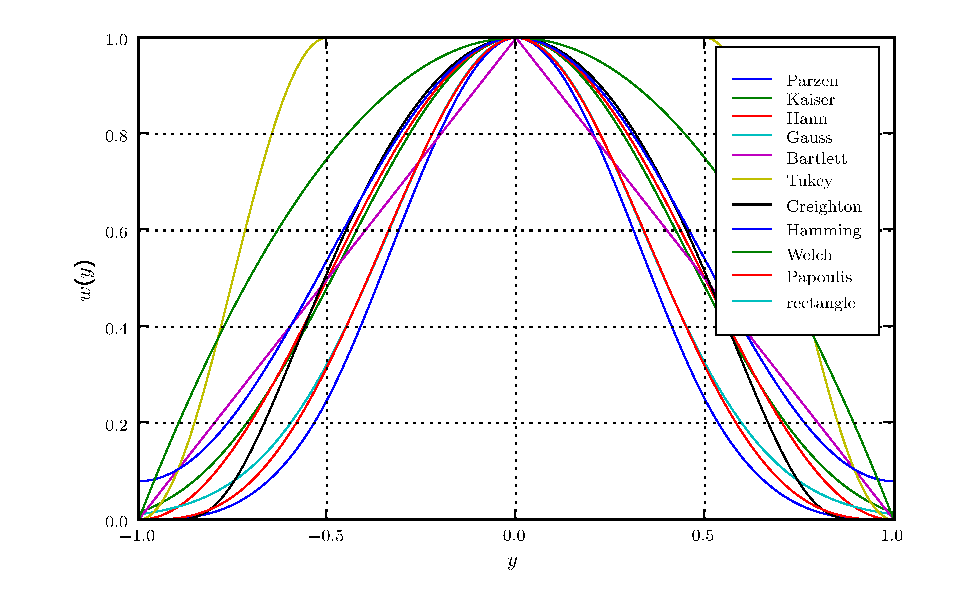
\includegraphics{window_t}
\end{center}
\caption{\label{f:window-t} Various windows as functions of the normalized
independend variable $y$, choosing $\beta = 6$ for the Kaiser window,
$\beta = 2$ for the Creighton window, $\beta = 0.5$ for the Tukey window,
and $\beta = 3$ for the Gauss window.}
\end{figure}

For a vector of length $L$ (an integer), the mapping from integer array
index $i$ to normalized co-ordinate $y$ is
\begin{equation}
y(i)
   = \left\{ \begin{array}{ll}
   0 & L \le 1, \\
   1 - 2 i / (L - 1) & L > 1,
   \end{array} \right.
\end{equation}
where $0 \le i < L$, and floating-point division is used.  This agrees with
J.~G.~Proakis and D.~G.~Manolakis, \textit{Digital Signal Processing}
\cite{pm}, and \texttt{MatLab}.  For odd-lengthed vectors, the middle
sample corresponds to $y = 0$, while for even-lengthed vectors $y = 0$
occurs half-way between the two middle samples.  Substituting $y(i)$ into
the definitions of the window functions above yields $w(i)$, the value of
the window function at the integer sample $i$.

The Fourier transforms of the windows are shown as functions of $1 / y$ in
Fig.~\ref{f:window-f}.
\begin{figure}
\begin{center}
\resizebox{0.6\textwidth}{!}{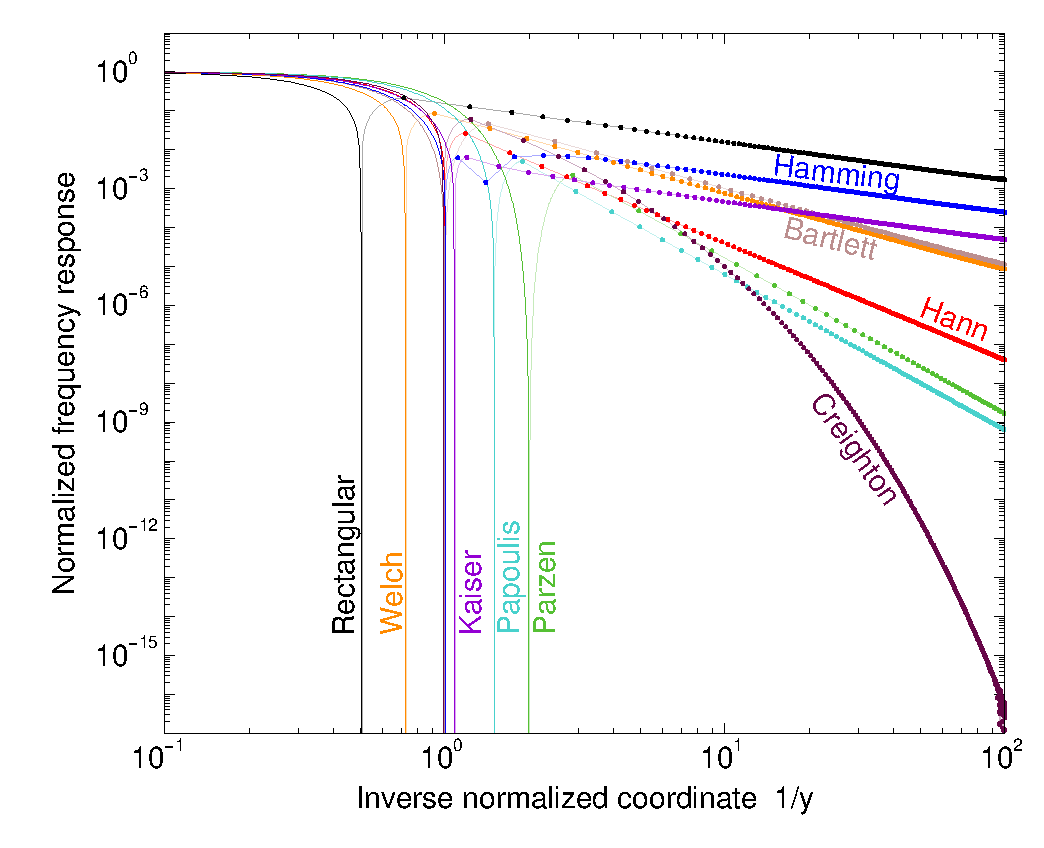
\includegraphics{window_f}}
\end{center}
\caption{\label{f:window-f} Frequency behaviour of various windows as
functions of the inverse of the normalized independend variable $y$,
choosing $\beta=6$ for Kaiser and $\beta=2$ for Creighton.  Solid lines
demark the central lobe, circles mark the peaks of the sidelobes.}
\end{figure}
Since the Fourier transform of windowed data is the Fourier transform of
the data convolved with the Fourier transform of the window,
Fig.~\ref{f:window-f} is the major guideline for selecting a window.  One
can see that windows with a narrow central lobe tend to have higher
sidelobes, and windows which suppress their low-order sidelobes tend to
have more power in the high-order sidelobes.  The choice of window thus
depends on whether one is trying to resolve nearby spectral features of
comparable magnitude (suggesting a rectangular or a Welch window), to
reduce spectral bias and low-order sidelobes (a Hamming or Kaiser window),
or to measure a broad spectrum with a large dynamical range (a Creighton or
a Papoulis window).


\begin{thebibliography}{0}
\bibitem{numrec}
W. H. Press, S. A. Teukolsky, W. T. Vetterling, and B. P. Flannery,
  \textit{Numerical Recipes in C: The Art of Scientific Computing}, 2nd ed.
  (Cambridge University Press, Cambridge, England, 1992).
\bibitem{pw}
D.B. Percival and A.T. Walden, {\it Spectral analysis for physical applications}, first edition, Cambridge University Press, (1993).
\bibitem{pm}
J.G. Proakis and D.G. Manolakis, {\it Digital
Signal Processing: principles, algorithms and applications},
3rd Edition, 1995.
Prentice Hall
\bibitem{stakgold}
I. Stakgold, {\it Green's Functions and Boundary Value Problems},
1979.
Wiley Interscience
\end{thebibliography}
